% IEEE Transactions on Artificial Intelligence version (IEEEtran journal mode).
% Build: cd paper/tai && python make_tai_figures.py && latexmk -pdf tai.tex
% Double-anonymous review: keep \anontrue for submission, \anonfalse for the camera-ready copy.
\documentclass[journal]{IEEEtran}
\usepackage[T1]{fontenc}
\usepackage{amsmath,amssymb,mathtools}
\let\proof\relax\let\endproof\relax
\usepackage{amsthm}
\usepackage{graphicx,booktabs,xcolor,enumitem}
\usepackage[numbers,sort&compress]{natbib}
\usepackage{xurl}
\usepackage[hidelinks]{hyperref}
\usepackage[capitalise,noabbrev]{cleveref}

\newif\ifanon\anontrue
\graphicspath{{figures/}{../figures/}}
% generated by paper/make_figures.py - do not edit
\newcommand{\NCal}{2179}
\newcommand{\NTest}{1566}
\newcommand{\NQwen}{1424}
\newcommand{\NIntern}{1333}
\newcommand{\NAmber}{1257}
\newcommand{\NSfive}{496}
\newcommand{\NAmberUnknown}{311}
\newcommand{\NAmberClaims}{1568}
\newcommand{\NTestHall}{395}
\newcommand{\NTestImg}{497}
\newcommand{\CleanClaim}{0.080}
\newcommand{\CleanImage}{0.100}
\newcommand{\CleanKept}{0.587}
\newcommand{\GdinoClaim}{0.609 [0.558, 0.657]}
\newcommand{\GdinoImage}{0.409 [0.365, 0.450]}
\newcommand{\GdinoRecClaim}{0.087 [0.060, 0.117]}
\newcommand{\GdinoRecImage}{0.083 [0.060, 0.107]}
\newcommand{\OwlvOneClaim}{0.012 [0.003, 0.023]}
\newcommand{\QwenClaim}{0.129 [0.094, 0.165]}
\newcommand{\InternClaim}{0.160 [0.112, 0.208]}
\newcommand{\QwenImage}{0.093 [0.070, 0.119]}
\newcommand{\InternImage}{0.074 [0.053, 0.098]}
\newcommand{\InternKeptHall}{0.042}
\newcommand{\CleanKeptHall}{0.044}
\newcommand{\AmberClaim}{0.036 [0.008, 0.074]}
\newcommand{\AmberImage}{0.007 [0.002, 0.014]}
\newcommand{\SfiveClaim}{0.105 [0.079, 0.132]}
\newcommand{\SfiveImage}{0.142 [0.112, 0.174]}
\newcommand{\NHtwo}{6}
\newcommand{\Jlearned}{0.14}
\newcommand{\LLgain}{5.45}
\newcommand{\CorrCal}{0.017}
\newcommand{\CorrTest}{0.015}
\newcommand{\AucUnary}{0.870}
\newcommand{\AucIsing}{0.871}
\newcommand{\RobEps}{0.910}
\newcommand{\RobB}{2.711}
\newcommand{\RobImgs}{150}
\newcommand{\WidthJ}{0.506}
\newcommand{\WidthJzero}{0.477}
\newcommand{\TanhJ}{0.139}
\newcommand{\ChairLlava}{0.145}
\newcommand{\ChairQwen}{0.091}
\newcommand{\ChairIntern}{0.076}
\newcommand{\TruncQwen}{47}
\newcommand{\HallRateLlava}{0.252}
\newcommand{\HallAboveLlava}{0.078}
\newcommand{\HallQninetyLlava}{-0.99}
\newcommand{\HallRateQwen}{0.211}
\newcommand{\HallAboveQwen}{0.126}
\newcommand{\HallQninetyQwen}{-0.69}
\newcommand{\HallRateIntern}{0.140}
\newcommand{\HallAboveIntern}{0.155}
\newcommand{\HallQninetyIntern}{-0.47}
\newcommand{\TauFull}{-0.879}
\newcommand{\MinKeptSone}{0.21}
\newcommand{\MinKeptSoneCond}{gaussian noise 5}
\newcommand{\MaxAbstSone}{0.48}
\newcommand{\MaxAbstSoneCond}{gaussian noise 5}
\newcommand{\NClaimPreservedSone}{25}
\newcommand{\NImagePreservedSone}{22}
\newcommand{\PtwoSlack}{0.25}
\newcommand{\ShareBgtEps}{1.00}
\newcommand{\GdinoKept}{0.970}
\newcommand{\GdinoRecKept}{0.599}
\newcommand{\InternKept}{0.602}

% generated by paper/tai/make_tai_figures.py - do not edit
\newcommand{\PiLlava}{0.469}
\newcommand{\RhoLlava}{0.213}
\newcommand{\PiQwen}{0.427}
\newcommand{\RhoQwen}{0.218}
\newcommand{\PiIntern}{0.286}
\newcommand{\RhoIntern}{0.260}
\newcommand{\RhoInternAtLlavaPi}{0.122}
\newcommand{\AlphaOverPiIntern}{0.350}
\newcommand{\AlphaOverPiLlava}{0.213}
\newcommand{\CorrLocal}{1.00}
\newcommand{\CorrGlobal}{0.75}
\newcommand{\MaxAbsLocalGap}{0.005}
\newcommand{\NSoneGlobalFail}{11}
\newcommand{\NLocalPoints}{27}
\newcommand{\LocalDeltaQwen}{+0.048}
\newcommand{\ExcessQwen}{+0.049}
\newcommand{\DplusQwen}{0.059}
\newcommand{\LocalDeltaIntern}{+0.077}
\newcommand{\ExcessIntern}{+0.080}
\newcommand{\DplusIntern}{0.090}
\newcommand{\BudgetTen}{170}
\newcommand{\BudgetFive}{290}
\newcommand{\BudgetTenEpsFive}{60}
\newcommand{\TailMFifty}{0.204}
\newcommand{\TailMHundred}{0.148}
\newcommand{\TailMTwoHundred}{0.082}
\newcommand{\TailMFiveHundred}{0.017}
\newcommand{\NormalApproxBudget}{164}


\newtheorem{theorem}{Theorem}
\newtheorem{corollary}{Corollary}
\newtheorem{proposition}{Proposition}
\theoremstyle{remark}\newtheorem{remark}{Remark}
\DeclareMathOperator{\Risk}{Risk}
\DeclareMathOperator{\Beta}{Beta}
\newcommand{\Sbar}{\bar F}
% TAI's own class provides IEEEImpStatement; plain IEEEtran does not.
\makeatletter
\@ifundefined{IEEEImpStatement}{\newenvironment{IEEEImpStatement}{\par\vspace{0.5ex}\noindent\bfseries\footnotesize\textit{Impact Statement}---}{\par\vspace{0.5ex}}}{}
\makeatother
\renewcommand{\Pr}{\mathbb{P}}
\newcommand{\E}{\mathbb{E}}
\newcommand{\repo}{\ifanon an anonymised repository (link withheld for review)\else
  \url{https://github.com/antonyjasfer/Budget-Coupled-Robust-Belief-Propagation-for-Visual-Hallucination-Detection}\fi}

\begin{document}
\title{When Do Conformal Hallucination Guarantees Survive Distribution Shift? Generator Change, Prevalence, and a Threshold-Local Condition}

\ifanon
\author{Anonymous Authors}
\else
\author{S.~Raja, A.~Antony~Selva~Jasfer, Akash~Narayanan~C, U.~Priyan, and Nisanth~S%
\thanks{S.~Raja is with the Department of Mathematics, Amrita School of Computing, Amrita Vishwa Vidyapeetham, Nagercoil 629001, India (e-mail: nellairajaa@yahoo.com).}%
\thanks{A.~Antony Selva Jasfer, Akash Narayanan C, U.~Priyan and Nisanth S are with the Department of Artificial Intelligence and Data Science, Amrita School of Computing, Amrita Vishwa Vidyapeetham, Nagercoil 629001, India.}}
\fi

\markboth{IEEE Transactions on Artificial Intelligence}{Conformal Hallucination Guarantees under Distribution Shift}

\maketitle

\begin{abstract}
Conformal filters remove object hallucinations from the captions of vision-language models (VLMs) by keeping a mentioned object only when an open-vocabulary detector finds enough evidence for it, and they promise that at most a chosen fraction of hallucinated mentions survives. The promise assumes that deployment data are exchangeable with the calibration data. We report a pre-registered audit of a claim-level and an image-level filter, calibrated once on COCO captions from LLaVA-1.5-7B scored by OWLv2, under 25 image corruptions, two detector swaps, two VLM swaps and a move to the AMBER benchmark. Image corruptions and the domain move left the claim-level risk within the pre-registered margin. Changing the caption generator did not: the claim-level risk rose to 0.160 on InternVL3-2B against a target of 0.10, while the image-level risk stayed at 0.074. We prove three results that explain this pattern. First, the realised risk under any shift equals the clean risk plus the expected change in the survival of hallucinated scores at the calibrated threshold, so preservation depends only on the shift near that threshold. Second, image-level risk factorises into hallucination prevalence times conditional survival, and the newer VLM passed only because it hallucinated in fewer captions; its hallucinations survived more often. Third, recalibrating on about 170 labelled hallucinated claims makes an overshoot of three points unlikely, by an exact Beta argument. A detector swap broke both filters and was repaired by rescoring the existing labelled claims.
\end{abstract}

\begin{IEEEImpStatement}
Systems that describe images in words are being used where false statements matter, such as accessibility tools and document processing. Statistical filters can remove invented objects with a stated error rate, but the rate is certified only for the conditions it was calibrated in. We show that the most common deployment change, replacing the language model that writes the descriptions, can quietly break that certificate while a stricter whole-image version appears to keep it. We explain why, give a check that needs no new labels, and say how many labelled examples restore the certificate. Practitioners can use these results to decide when a filter must be recalibrated, and auditors can use them to test claims about filtered systems. The study uses public benchmarks and open models only.
\end{IEEEImpStatement}

\begin{IEEEkeywords}
Conformal prediction, distribution shift, object hallucination, vision-language models, risk control, pre-registration.
\end{IEEEkeywords}

% ===================================================================== I
\section{Introduction}\label{sec:intro}
\IEEEPARstart{V}{ision-language} models (VLMs) write fluent image descriptions that often mention objects which are not there. CHAIR measures this object hallucination by comparing the objects named in a caption with the objects annotated in the image \cite{rohrbach2018chair}, and benchmarks such as POPE and AMBER probe it in other ways \cite{li2023pope,wang2023amber}. A practical defence checks every mentioned object against independent visual evidence, usually an open-vocabulary detector, and removes what the evidence does not support. CEBC sets the detector threshold at the $(1-\delta)$ quantile of the scores of hallucinated mentions in a calibration set \cite{cebc}, and ConfLVLM filters claims so that a retained answer is correct with probability at least $1-\alpha$ \cite{conflvlm}. With split conformal calibration, both kinds of filter carry finite-sample guarantees that need no model of the VLM or the detector \cite{vovk2005algorithmic,angelopoulos2023gentle}.

Those guarantees assume that deployment data are exchangeable with the calibration data. That conformal factuality can fail when this assumption breaks is now established for text-only language models. Chen et al.\ find it ``is not robust to distribution shifts'' in retrieval-augmented generation, including when calibration claims come from a different generator \cite{chen2026conformalrag}. Zhu et al.\ show that changing the prompt template, decoding temperature or quantization erodes coverage, bound the loss by a discrepancy between calibration and test scores, and recalibrate with a few labelled examples \cite{zhu2026configuration}. CoFact reweights calibration data under covariate shift \cite{hu2026cofact}. For VLMs, BCEA notes that reusing a threshold after its own re-examination step breaks its bound \cite{xu2026bcea}, and IntroConformal states that model updates ``require recalibration'' \cite{atabuzzaman2026introconformal}. None of these studies asks which deployment changes break a detector-evidence filter for VLMs, or why one formulation of the guarantee can survive a change that breaks another.

We answer these questions with a pre-registered audit and three short theorems. The audit calibrates a CEBC-style claim-level filter and a ConfLVLM-style image-level filter once, on clean COCO captions from LLaVA-1.5-7B scored by OWLv2, and exposes them to five families of shift (\cref{fig:pipeline}). Our contributions are as follows.
\begin{enumerate}[leftmargin=*,itemsep=1pt,topsep=2pt]
\item \emph{Generator change is the dangerous shift.} Image corruptions and a partial domain shift kept the claim-level risk within its pre-registered margin. Replacing LLaVA-1.5-7B with InternVL3-2B raised it to \InternClaim{} against a target of 0.10, and Qwen2.5-VL-3B was inconclusive at \QwenClaim{}. A detector swap also broke both filters, but rescoring the existing labelled claims repaired it without new annotation.
\item \emph{A threshold-local identity} (\cref{thm:local}). The realised risk under any shift equals the clean risk plus the expected change, at the calibrated threshold, in the probability that a hallucinated claim scores above it. Global stochastic dominance, the condition of our pre-registered hypothesis H2, is sufficient but held in only \NHtwo{} of 25 corruptions; the local change accounts for all of them and for both VLM swaps.
\item \emph{A prevalence decomposition} (\cref{thm:prev}). Image-level risk is the share of captions that contain a hallucination times the probability that such a caption keeps one. InternVL3-2B passed at image level because it hallucinated in fewer captions (\PiIntern{} against \PiLlava{}), not because its hallucinations were easier to catch: they survived more often (\RhoIntern{} against \RhoLlava{}). At LLaVA's prevalence the same tail would give \RhoInternAtLlavaPi{}.
\item \emph{A label budget for repair} (\cref{thm:budget}). Recalibrating on $m$ labelled hallucinated claims gives a realised risk with an exact Beta law; $m\ge\BudgetTen$ keeps the probability of exceeding $0.13$ at or below $0.10$.
\end{enumerate}
We also report a negative result on modelling a caption's claims jointly: a root-dominance bound for Ising trees shows why coupling claims cannot narrow robust intervals at the measured coupling (\cref{app:ising}).

\begin{figure}[t]
\centering
\includegraphics[width=\linewidth]{col_pipeline.png}
\caption{Setting of the audit. A VLM describes an image; each object it mentions is a claim. A detector scores every claim, and a claim is kept only if its score exceeds a threshold calibrated once on clean data. Labels mark where each family of shift enters.}
\label{fig:pipeline}
\end{figure}

% ===================================================================== II
\section{Related Work}\label{sec:related}
\emph{Measuring and detecting hallucination.} CHAIR counts COCO objects \cite{lin2014microsoft} that a caption names but the image annotations lack \cite{rohrbach2018chair}; it is our labelling rule, and it is known to miss some hallucinations \cite{petryk2024aloha}. POPE asks yes/no questions about objects \cite{li2023pope}, and AMBER annotates present objects and likely ``hallucinatory target'' objects without an LLM in the loop \cite{wang2023amber}. Detection methods score claims with answer uncertainty \cite{zhang2024vluncertainty}, attention drift \cite{wen2026cadmp}, Bayesian combinations of internal signals \cite{zohrabi2026haloprobe}, or evidential conflict \cite{huang2025evidential}. They produce scores; we study the guarantee attached to a score.

\emph{Conformal guarantees for generated content.} Split conformal prediction \cite{vovk2005algorithmic,angelopoulos2023gentle} and conformal risk control \cite{angelopoulos2022conformal} underlie claim filtering for language models \cite{mohri2024language,cherian2024large} and VLMs \cite{conflvlm,cebc,xu2026bcea,atabuzzaman2026introconformal}. All of these state their guarantees for exchangeable or i.i.d.\ data. We found no public code for CEBC, ConfLVLM or BCEA, so our filters are re-implementations of their thresholding steps, which we call CEBC-style and ConfLVLM-style.

\emph{Conformal prediction under shift.} Weighting restores validity under covariate shift with a known likelihood ratio \cite{tibshirani2019covariate}; without exchangeability the coverage gap is bounded by total-variation terms \cite{barber2023beyond}; robust variants cover an $f$-divergence ball \cite{cauchois2024robust} or bounded input perturbations \cite{gendler2022adversarially}. These need the form and size of the shift in advance. One-sided comparisons of score distributions describe when transported or contaminated calibration stays valid \cite{doula2026conformal,clarkson2024split,lee2026diagnosing}, and Zhu et al.\ bound the gap by a global score discrepancy \cite{zhu2026configuration}. \cref{thm:local} is an exact, local and one-sided identity in the same spirit, applied to the scores of hallucinated claims only; \cref{thm:prev,thm:budget} have no counterpart in these works that we know of.

% ===================================================================== III
\section{Setting}\label{sec:setting}
\emph{Claims and scores.} A VLM writes a caption for an image. Following CHAIR, every COCO category the caption mentions is a claim, hallucinated ($Y=1$) if the category is not among the image's annotated objects and supported ($Y=0$) otherwise. A detector is queried with ``a photo of a $\langle$category$\rangle$''; the logit of its highest box probability is the claim's score $S$.

\emph{Claim-level filter.} Let $S_1,\dots,S_n$ be the scores of hallucinated calibration claims. The filter keeps a claim if its score exceeds
\begin{equation}\label{eq:tau}
\hat\tau=S_{(k)},\qquad k=\lceil (n+1)(1-\delta)\rceil ,
\end{equation}
the $k$-th smallest score ($\hat\tau=+\infty$ if $k>n$). Its risk is $R_c=\Pr(S>\hat\tau\mid Y=1)$, the probability that a hallucinated test claim survives. This is CEBC's threshold \cite{cebc} with the finite-sample index of split conformal prediction and without clipping; we study only the filtering step.

\emph{Image-level filter.} For an image let $K$ be its number of hallucinated claims and $M$ the largest of their scores ($M=-\infty$ if $K=0$). The threshold $\hat\tau_I$ is \eqref{eq:tau} applied to $M_1,\dots,M_n$ over calibration images with $1-\alpha$ in place of $1-\delta$, and the risk is $R_I=\Pr(M>\hat\tau_I)$, the probability that an image keeps a hallucination. This is ConfLVLM's guarantee with zero tolerance \cite{conflvlm}, computed from CHAIR labels and detector scores rather than from its own claim decomposition and confidence scores.

\emph{The exchangeable unit.} Images are split into calibration and test sets at random, so the image is the exchangeable unit and $R_I\le\alpha$ holds exactly in finite samples \cite{vovk2005algorithmic}. Claims within an image are dependent, so a pooled hallucinated claim is not exchangeable with the calibration claims and $R_c\le\delta$ holds only approximately; exact grouped versions exist \cite{dunn2023hierarchical,lee2026hierarchical}. We keep the pooled form because it is CEBC's. Both risks are unconditional, averaged over the draw of the calibration set. We use $\delta=\alpha=0.10$.

% ===================================================================== IV
\section{Theory}\label{sec:theory}
Write $P$ for the distribution of the score of a hallucinated claim in the clean (calibration) regime and $Q$ for its distribution after a shift, with survival functions $\Sbar_P(t)=P(S>t)$ and $\Sbar_Q(t)=Q(S>t)$, and let
\begin{equation}\label{eq:delta}
\Delta(t)=\Sbar_Q(t)-\Sbar_P(t)
\end{equation}
be the change in survival at height $t$. The calibration sample, and so $\hat\tau$, is drawn from $P$; the test claim is drawn from $Q$, independently. The results apply to any exchangeable unit: to claims under the idealisation that hallucinated claims are i.i.d., and exactly to images with $M$ in place of $S$.

\begin{theorem}[Threshold-local identity]\label{thm:local}
Let $P$ be continuous and $1\le k\le n$. Then
\begin{equation}\label{eq:local}
\Risk_Q=\Pr_Q(S>\hat\tau)=1-\frac{k}{n+1}+\E\,\Delta(\hat\tau).
\end{equation}
(a) Hence $\Risk_Q\le\delta$ if and only if $\E\,\Delta(\hat\tau)\le s_n$, where $s_n=\delta-1+k/(n+1)\in[0,1/(n+1))$ is the slack of the clean filter.
(b) If $\Delta(t)\le0$ for all $t$, the guarantee is preserved.
(c) If $P$ has a continuous positive density at its $(1-\delta)$ quantile $q$ and $\Delta$ is continuous at $q$, then $\Risk_Q\to\delta+\Delta(q)$ as $n\to\infty$.
\end{theorem}
Part (b) is the global dominance condition tested by hypothesis H2. Part (a) is the point: preservation is decided by $\Delta$ near the threshold, averaged over its sampling distribution, and nowhere else. A shift may raise hallucinated scores far above or below $\hat\tau$ without consequence, which is why global dominance is sufficient but far from necessary. Part (c) says that, for large calibration sets, the guarantee asymptotically survives exactly when $\Delta(q)\le0$. Given $m$ labelled shifted hallucinated claims, the realised risk at the fixed threshold $\hat\tau$ can be certified with any one-sided binomial upper bound, because those claims are independent of $\hat\tau$. Proofs are in \cref{app:proofs}.

\begin{theorem}[Prevalence decomposition]\label{thm:prev}
For an image, let $\pi=\Pr(K\ge1)$ and $\rho(t)=\Pr(M>t\mid K\ge1)$. Then for every threshold $t$
\begin{equation}\label{eq:prev}
\Pr(M>t)=\pi\,\rho(t).
\end{equation}
(a) After a change of generator from $P$ to $Q$, the image-level guarantee calibrated on $P$ is preserved if and only if $\E\,\rho_Q(\hat\tau_I)\le\alpha/\pi_Q$.
(b) If, given $K=j$, the $j$ hallucinated scores are i.i.d.\ with survival $\Sbar$, then $\rho(t)=1-\sum_{j\ge1}\Pr(K=j\mid K\ge1)\,(1-\Sbar(t))^{j}$, which increases with both $\Sbar(t)$ and $K$.
(c) Consequently, a generator with lower prevalence can pass at image level while its hallucinations survive more often, and image-level and claim-level verdicts can disagree in either direction.
\end{theorem}
The condition in (a) loosens as $\pi_Q$ falls: a generator that hallucinates in fewer captions is shielded at image level, whatever happens to the scores of the hallucinations it does make. \Cref{sec:res-prev} shows this happened in our audit.

\begin{theorem}[Label budget for recalibration]\label{thm:budget}
Let $T_1,\dots,T_m$ be i.i.d.\ scores of labelled hallucinated claims from a continuous shifted distribution $Q$, let $k=\lceil(m+1)(1-\delta)\rceil\le m$ and $\hat\tau_m=T_{(k)}$. Conditionally on the sample, the realised risk $R_m=\Sbar_Q(\hat\tau_m)$ satisfies
\begin{equation}\label{eq:beta}
R_m\sim\Beta(m+1-k,\,k),\qquad \E R_m=\frac{m+1-k}{m+1}\le\delta .
\end{equation}
\end{theorem}
This is the training-conditional law of split conformal prediction \cite{vovk2012conditional} applied to recalibration. It turns ``how many labels do we need'' into an exact computation. For $\delta=0.10$ and an overshoot of $\varepsilon=0.03$, $\Pr(R_m>0.13)$ falls at or below $0.10$ for every $m\ge\BudgetTen$ and at or below $0.05$ for $m\ge\BudgetFive$ (\cref{fig:budget}); with $\varepsilon=0.05$, $m\ge\BudgetTenEpsFive$ suffices. The normal approximation gives \NormalApproxBudget. The curve is a saw-tooth because $k$ jumps by one as $m$ grows.

% ===================================================================== V
\section{Pre-Registered Design}\label{sec:design}
\emph{Pre-registration.} Hypotheses, decision rules, shift parameters and analysis code were frozen under the git tag prereg-v2 in \repo{} before any test caption or score existed, and the tests were run once. Pilots on 200 development images, kept apart from calibration and test, motivated the hypotheses and are excluded by code. \Cref{thm:local,thm:prev,thm:budget} and the analyses that use them were added after the confirmatory tests and are exploratory.

\emph{Data and pipeline.} COCO val2014 \cite{lin2014microsoft} was split with a fixed seed into 700 calibration images (\NCal{} claims) and a locked test set of 500 images; the \NTestImg{} test images that produced a claim gave \NTest{} claims, \NTestHall{} hallucinated. Captions come from LLaVA-1.5-7B \cite{liu2024improved} (greedy decoding, prompt ``Please describe this image in detail.'', at most 512 new tokens), claims from our re-implementation of CHAIR with its official synonym list, and scores from OWLv2 \cite{minderer2023scaling}. All GPU work ran on two NVIDIA T4 GPUs; the analysis was re-run from raw files on a second machine with identical results.

\emph{Shifts}, applied to test data only, one at a time. S1: five corruptions at five severities each \cite{hendrycks2019benchmarking}. S2: OWLv2 replaced by OWL-ViT v1 \cite{minderer2022simple} or Grounding DINO \cite{liu2024grounding}, with and without recalibration on the same labelled calibration claims, which needs no new labels because a claim's label does not depend on the detector. S3: LLaVA replaced by Qwen2.5-VL-3B \cite{bai2025qwen25} or InternVL3-2B \cite{zhu2025internvl3} with the same prompt and decoding. S4: 804 AMBER images \cite{wang2023amber}, labelled with AMBER's annotated present and hallucinatory-target lists (\NAmberUnknown{} of \NAmberClaims{} claims in neither list excluded); some AMBER images come from COCO, so this shift is partial. S5 (exploratory): one supported object per image painted over with the image's mean colour.

\emph{Hypotheses and decisions.} H1: every S1 condition preserves both targets. H2: under S1, hallucinated scores are stochastically no larger than clean ones. H3: some S2 swap violates the claim-level target. H4: recalibration repairs every swap. H5: thresholds transfer to each S3 VLM. H6: they transfer to AMBER. Risks are averaged over 200 calibration resamples of 80\% of the calibration images, with 95\% intervals from a 2,000-sample image-level cluster bootstrap \cite{efron1993introduction}. A condition is \emph{violated} if its interval lies above the target, \emph{preserved} if its upper bound is at most the target plus 0.03, and \emph{inconclusive} otherwise; Holm-adjusted bootstrap tail shares \cite{holm1979simple} are reported as a secondary summary.

\emph{Power.} With \NTestHall{} hallucinated test claims the binomial half-width of a 95\% interval near 0.10 is about 0.03, comparable to the margin. The design therefore separates large effects, such as the detector swap, from small ones only coarsely; Qwen2.5-VL-3B (301 hallucinated claims) and InternVL3-2B (187) are less powered still. We return to this in \cref{sec:limits}.

% ===================================================================== VI
\section{Results}\label{sec:results}
\Cref{tab:main} gives every shift except the corruptions, which \cref{fig:local} summarises; the pre-registered verdicts were H1 supported at claim level only, H2 not supported, H3 and H4 supported, H5 not supported at claim level, and H6 supported.

\begin{table*}[t]
\centering
\caption{Shifts other than corruption (target 0.10): risk [95\% interval], pre-registered decision, share of supported claims kept, and image-level abstention}
\label{tab:main}
\begin{tabular}{@{}lllllll@{}}\toprule
Condition & Claim-level risk & Decision & Image-level risk & Decision & Kept & Abstained\\\midrule
Clean (reference) & 0.080 [0.057, 0.106] & preserved & 0.100 [0.075, 0.126] & preserved & 0.587 & 0.030 \\
Detector: OWL-ViT v1 & 0.012 [0.003, 0.023] & preserved & 0.019 [0.008, 0.031] & preserved & 0.524 & 0.103 \\
OWL-ViT v1, recalibrated & 0.030 [0.015, 0.046] & preserved & 0.041 [0.026, 0.059] & preserved & 0.606 & 0.069 \\
Detector: Grounding DINO & 0.609 [0.558, 0.657] & \textbf{violated} & 0.409 [0.365, 0.450] & \textbf{violated} & 0.970 & 0.000 \\
Grounding DINO, recalibrated & 0.087 [0.060, 0.117] & preserved & 0.083 [0.060, 0.107] & preserved & 0.599 & 0.036 \\
VLM: Qwen2.5-VL-3B & 0.129 [0.094, 0.165] & \emph{inconcl.} & 0.093 [0.070, 0.119] & preserved & 0.604 & 0.060 \\
VLM: InternVL3-2B & 0.160 [0.112, 0.208] & \textbf{violated} & 0.074 [0.053, 0.098] & preserved & 0.602 & 0.048 \\
Domain: AMBER & 0.036 [0.008, 0.074] & preserved & 0.007 [0.002, 0.014] & preserved & 0.683 & 0.152 \\
Object removed (S5, exploratory) & 0.105 [0.079, 0.132] & \emph{inconcl.} & 0.142 [0.112, 0.174] & \textbf{violated} & -- & 0.858 \\
\bottomrule

\end{tabular}
\end{table*}

\subsection{Changing the generator breaks the claim-level guarantee}\label{sec:res-gen}
Thresholds calibrated on LLaVA did not transfer at claim level: InternVL3-2B was violated at \InternClaim{} and Qwen2.5-VL-3B was inconclusive at \QwenClaim{}. The image-level filter was preserved for both, at \InternImage{} and \QwenImage{}. The newer VLMs hallucinate less often (\HallRateIntern{} and \HallRateQwen{} of their claims, against \HallRateLlava{} for LLaVA), but the hallucinations they make sit higher on OWLv2's scale: the 90th percentile of their scores is \HallQninetyIntern{} and \HallQninetyQwen{} logits, against \HallQninetyLlava{} (\cref{fig:vlm}). In terms of \cref{thm:local}, the change in survival at the threshold was \LocalDeltaIntern{} for InternVL3-2B and \LocalDeltaQwen{} for Qwen2.5-VL-3B, and the realised excess risks were \ExcessIntern{} and \ExcessQwen{}.

\begin{figure}[t]
\centering
\includegraphics[width=\linewidth]{col_vlm.png}
\caption{Survival of OWLv2 scores of hallucinated test claims for each VLM, with the threshold calibrated on LLaVA (dashed). The newer VLMs' hallucinations cross it more often. Exploratory.}
\label{fig:vlm}
\end{figure}

\subsection{Image-level robustness is a prevalence effect}\label{sec:res-prev}
\Cref{thm:prev} splits each image-level risk into prevalence and conditional survival (\cref{fig:prev}). LLaVA-1.5-7B hallucinated in \PiLlava{} of the test images that produced claims, Qwen2.5-VL-3B in \PiQwen{} and InternVL3-2B in \PiIntern{}. The probability that an image with a hallucination kept one was \RhoLlava, \RhoQwen{} and \RhoIntern{}. InternVL3-2B's hallucinations therefore survived the image-level filter more often than LLaVA's, as they did at claim level, and its image-level risk stayed below 0.10 only because fewer of its captions contained a hallucination at all. Had it hallucinated as often as LLaVA, the same conditional survival would have given an image-level risk of \RhoInternAtLlavaPi{}. The image-level guarantee did not survive the generator change because it is more robust in kind; it survived because the new generator was more accurate, and a less accurate generator with the same score tail would break it.

\begin{figure}[t]
\centering
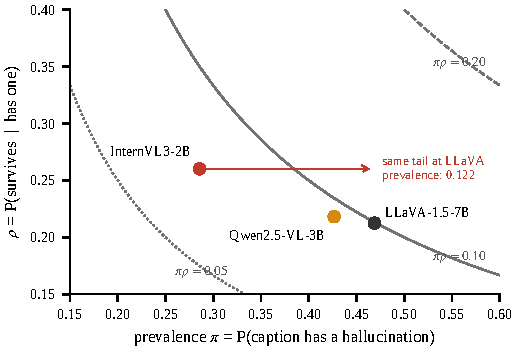
\includegraphics[width=\linewidth]{fig_prevalence.pdf}
\caption{Prevalence decomposition of image-level risk (\cref{thm:prev}). Curves show $\pi\rho$ equal to 0.05, 0.10 and 0.20; points are the three VLMs, coloured by their claim-level decision. Exploratory; $\rho$ is the image-level risk divided by $\pi$.}
\label{fig:prev}
\end{figure}

\subsection{Corruptions are safe because the change at the threshold is small}\label{sec:res-s1}
All 25 corruptions were preserved at claim level, with every point estimate at most 0.096; at image level three mild ones were inconclusive, just above the margin. Corruption lowers the detector's evidence for every object, so risk mostly fell as severity rose, at a cost in utility: under the strongest Gaussian noise the claim-level filter kept only \MinKeptSone{} of supported claims. The pre-registered H2, global dominance, failed in 19 of the 25 conditions: mild JPEG, noise and contrast raised some hallucinated scores somewhere. \Cref{fig:local} shows why that did not matter. The global gap $D^+=\max_t\Delta(t)$ is a poor guide to the realised excess risk (correlation \CorrGlobal), while the change at the calibrated threshold reproduces it to within \MaxAbsLocalGap{} across all \NLocalPoints{} corruption and generator conditions, as \eqref{eq:local} requires. The agreement is a consistency check of the identity, not independent evidence; its content is that only the local change matters.

\begin{figure}[t]
\centering
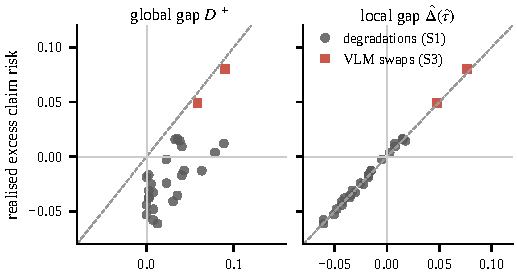
\includegraphics[width=\linewidth]{fig_local.pdf}
\caption{Realised excess claim-level risk against the global one-sided gap $D^+$ (left, the statistic of hypothesis H2) and against the change in survival at the calibrated threshold (right, \cref{thm:local}). Dashed: identity line.}
\label{fig:local}
\end{figure}

\subsection{A detector swap breaks both filters; rescoring repairs it}
Replacing OWLv2 with Grounding DINO raised the claim-level risk to \GdinoClaim{} and the image-level risk to \GdinoImage{}. Its scores lie on a different scale and are high even for absent objects, so almost every claim cleared the old threshold and \GdinoKept{} of supported claims were kept. This failure is the least surprising of our results, because a threshold is a property of a score scale. It is also the cheapest to repair: rescoring the same labelled calibration claims with Grounding DINO restored both targets (\GdinoRecClaim{} and \GdinoRecImage{}). OWL-ViT v1 made the filters conservative (\OwlvOneClaim{}).

A generator change cannot be repaired this way, because the hallucinations of the new generator are new claims that need labels. \Cref{thm:budget} says how many. With \BudgetTen{} labelled hallucinated claims from the new generator, the recalibrated filter overshoots 0.13 with probability at most 0.10; with 50 it does so with probability \TailMFifty{}, and with 100 with probability \TailMHundred{} (\cref{fig:budget}). At InternVL3-2B's hallucination rate, \BudgetTen{} hallucinated claims correspond to roughly 1,200 claims to label.

\begin{figure}[t]
\centering
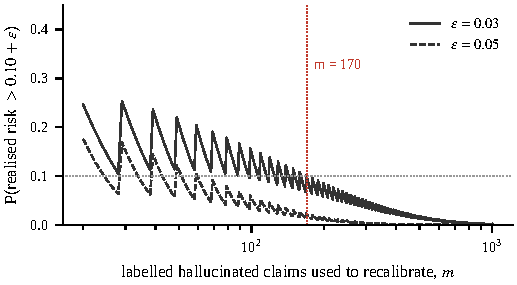
\includegraphics[width=\linewidth]{fig_budget.pdf}
\caption{Probability that a filter recalibrated on $m$ labelled hallucinated claims has realised risk above $0.10+\varepsilon$ (\cref{thm:budget}). The dotted line marks the smallest $m$ beyond which it stays at or below 0.10 for $\varepsilon=0.03$.}
\label{fig:budget}
\end{figure}

\subsection{Domain shift and object removal}
On AMBER both filters were preserved and conservative (\AmberClaim{} at claim level, \AmberImage{} at image level). In the exploratory object-removal test, the filter still kept the painted-over object's claim with probability \SfiveClaim{}, which suggests that the detector can still see the object's outline or context.

% ===================================================================== VII
\section{Discussion}\label{sec:discussion}
\emph{A recipe.} Changes to the images, as in corruption and the partial domain shift, did not break the filters; changes to the pipeline did. Before deploying a calibrated filter with a new detector, rescore the labelled calibration claims and recalibrate; this costs no annotation. Before deploying it behind a new generator, estimate the change in survival at the calibrated threshold on a small labelled sample (\cref{thm:local}); if it is positive, label about \BudgetTen{} hallucinated claims from the new generator and recalibrate (\cref{thm:budget}). Do not read a preserved image-level guarantee as evidence that the claim-level one also holds, or that the image-level one will hold for a generator that hallucinates more often (\cref{thm:prev}).

\emph{Which guarantee to report.} The claim-level risk is the probability that a hallucination survives; the image-level risk is the probability that an output contains one. Neither is the share of hallucinated claims among those kept, which is what a reader experiences; that share was \InternKeptHall{} for InternVL3-2B against \CleanKeptHall{} for LLaVA. Learn-then-test procedures can control that share directly, and we leave their behaviour under shift to future work.

\emph{Limitations.}\label{sec:limits} Our evidence covers one source pipeline, three generators and three detectors, with test sets that are small for the effects at stake; the InternVL3-2B violation rests on 187 hallucinated claims. Labels come from CHAIR on COCO's 80 categories, which miss some hallucinations \cite{petryk2024aloha}, and no human audit of labels has yet been done. Our filters re-implement only the thresholding steps of CEBC and ConfLVLM. COCO images may appear in the training data of the VLMs and detectors. \Cref{thm:local,thm:prev,thm:budget} were derived after the pre-registered tests, and the analyses that use them are exploratory; the claim-level versions rest on treating hallucinated claims as i.i.d., which they are not within an image. A pre-registered extension with more generators and detectors, larger test sets, a human label audit and grouped conformal variants is planned.

% ===================================================================== VIII
\section{Conclusion}
Conformal hallucination filters for VLMs keep their guarantee under image corruption and a partial domain shift but lose it when the generator changes, and the image-level guarantee that appeared to survive did so because the new generator hallucinated in fewer captions. Whether a guarantee survives is decided by the change in survival of hallucinated scores at the calibrated threshold, and a few hundred labelled hallucinated claims restore it. A detector change, by contrast, can be repaired for free by rescoring the existing labelled claims.

\section*{Data and Code Availability}
Code, the pre-registration (tag prereg-v2), raw captions and detector scores, and the scripts that produce every number and figure are in \repo{}\ifanon\else{} and on Zenodo (\url{https://doi.org/10.5281/zenodo.23810032})\fi, under the MIT licence for code and CC BY 4.0 for data.

% Acknowledgment / AI-use disclosure: IEEE asks authors to disclose AI-generated content in the
% acknowledgments section. Decide the wording with all authors before submission.

\appendices
\section{Proofs}\label{app:proofs}
\begin{proof}[Proof of \cref{thm:local}]
The test claim is independent of $\hat\tau$, so $\Pr_Q(S>\hat\tau)=\E\,\Sbar_Q(\hat\tau)=\E\,\Sbar_P(\hat\tau)+\E\,\Delta(\hat\tau)$. With $U_i=F_P(S_i)$ i.i.d.\ uniform, $\Sbar_P(\hat\tau)=1-U_{(k)}$ and $\E U_{(k)}=k/(n+1)$, which gives \eqref{eq:local}. Part (a) is a rearrangement, and $s_n\in[0,1/(n+1))$ because $(n+1)(1-\delta)\le k<(n+1)(1-\delta)+1$. Part (b) follows from (a) and $s_n\ge0$. For (c), $k/(n+1)\to1-\delta$, and under the density assumption the sample quantile $\hat\tau\to q$ in probability; $\Delta$ is bounded and continuous at $q$, so $\E\,\Delta(\hat\tau)\to\Delta(q)$ by bounded convergence.
\end{proof}
\begin{proof}[Proof of \cref{thm:prev}]
$\{M>t\}\subseteq\{K\ge1\}$ because $M=-\infty$ when $K=0$, so $\Pr(M>t)=\Pr(K\ge1)\Pr(M>t\mid K\ge1)$. Part (a) applies this to $Q$ at the threshold $\hat\tau_I$, which is independent of the test image, and takes expectations. For (b), given $K=j$ the maximum of $j$ i.i.d.\ scores exceeds $t$ unless all $j$ fall at or below $t$, which has probability $(1-\Sbar(t))^j$; average over $j$ given $K\ge1$. Each term increases in $\Sbar(t)$ and in $j$. Part (c) follows from (a) and (b): $\rho_Q$ can exceed $\rho_P$ while $\pi_Q\rho_Q<\pi_P\rho_P$.
\end{proof}
\begin{proof}[Proof of \cref{thm:budget}]
With $V_i=\Sbar_Q(T_i)$, the $V_i$ are i.i.d.\ uniform because $Q$ is continuous, and $\Sbar_Q$ is non-increasing, so $R_m=\Sbar_Q(T_{(k)})=V_{(m+1-k)}$, the $(m+1-k)$-th smallest of $m$ uniforms, which is $\Beta(m+1-k,k)$. Its mean is $(m+1-k)/(m+1)\le\delta$ by the choice of $k$.
\end{proof}

\section{A Negative Result on Coupling Claims}\label{app:ising}
One might hope to make a filter more robust by modelling a caption's claims jointly. We modelled the labels $h_i\in\{-1,+1\}$ of an image's claims ($+1$ hallucinated) as an attractive Ising tree, $p(h)\propto\exp(\sum_i\theta_ih_i+\sum_{(i,j)}J_{ij}h_ih_j)$ with $J_{ij}\ge0$, and asked how far the posterior log-odds field $\eta_r$ of a target claim can move when the fields $\theta_i$ are perturbed by $|\delta_i|\le\varepsilon_i$ with $\sum_i|\delta_i|\le B$. Let $\gamma_i$ be the product of $\tanh J_e$ along the path from claim $i$ to $r$ and $\gamma_{\max}<1$ its largest value.

\begin{proposition}[Root dominance]\label{prop:ising}
With $a=\min(\varepsilon_r,B)$, the largest reachable field satisfies $\eta_r+a\le\eta_r^{\sup}\le\eta_r+a+\gamma_{\max}\max(0,B-\varepsilon_r)$, and symmetrically for the smallest. If $B\le\varepsilon_r$ the robust interval for $\Pr(h_r=+1)$ is exactly $[\sigma(2(\eta_r-B)),\sigma(2(\eta_r+B))]$, whatever the graph.
\end{proposition}
The proof combines the structure-free gain bound of Chan and Darwiche \cite{chan2002numbers} with the Ising case of the message contraction of Ihler et al.\ \cite{ihler2005loopy} and is in the supplement. The statement is about the log-odds field; because $\sigma$ is monotone the interval follows, but widths in probability depend on where $\eta_r$ sits. In our data the claims of a caption were almost uncorrelated (\CorrTest), the learned chain coupling was $J=\Jlearned$, coupling left test ROC-AUC unchanged (\AucIsing{} against \AucUnary), and robust intervals were wider with it (\WidthJ{} against \WidthJzero), as the proposition predicts: coupling adds a channel for perturbation and never removes the target's own.

\bibliographystyle{IEEEtranN}
\bibliography{../refs}
\end{document}
